\section{What the numbers in Panel B are}

Every cell holds two numbers separated by a slash. The second one is easy: it is the raw coverage,
the fraction of problems on which the interval the procedure actually reported contained the true
causal effect. The first one is the whole design of the table, and it is not a width in effect units.
It is the answer to this question:

\begin{quoting}
\emph{If we forced this procedure to be honest, how wide would it have to be, compared with the
width that throwing the knowledge away would need?}
\end{quoting}

The reason the table is built that way is that a raw width and a raw coverage, printed as two free
columns, let any procedure shelter in one of them. Discarding the knowledge and reporting the
interval over every graph the data allows covers the truth essentially always, in every regime. It
passes any coverage gate that could be written. So the argument has to happen in the width column,
and a width column is only meaningful between procedures that cover equally. Calibrating first, then
measuring width, is what makes the comparison fair.

\subsection{Step 1. How far off is one reported interval}

Take a single problem at a single sample: a network, a treatment, an outcome, one random draw of
data. The procedure reports an interval. It has a midpoint and a half-width. The true effect is
known, because the data was generated from a graph we hold.

Measure the distance from the interval's midpoint to the truth, in units of the interval's own
half-width. Call it $\lambda_i$. A value below one means the interval already contains the truth.
A value of exactly one means it reaches it at the endpoint. A value of three means the interval
would have to be made three times wider, about its own midpoint, before it touched the truth.

\begin{figure}[h]
\centering
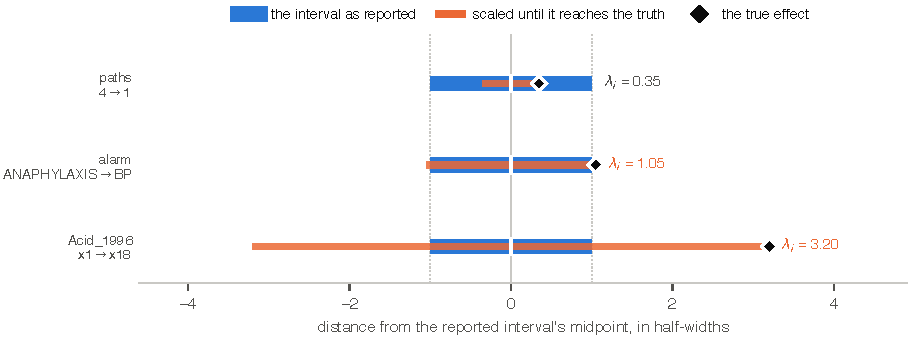
\includegraphics[width=\textwidth]{figs/f1_lambda.pdf}
\caption{Three real problems from the one-wrong-claim condition, at $n = 1000$, drawn on a common
scale where the reported interval always runs from $-1$ to $+1$. The factor $\lambda_i$ is what the
interval would have to be multiplied by, about its own midpoint, to reach the true effect.}
\end{figure}

\subsection{Step 2. One factor for the whole cell}

Now do that for every problem in the cell and every random draw. A cell of Panel B at one wrong
claim holds 359 problems and twenty draws each, so 7{,}180 of these numbers.

Sort them and take the 95th percentile. Call it $\lambda^{*}$. By construction, multiplying every
interval in the cell by $\lambda^{*}$ makes 95\,\% of them contain the truth. That is the single
factor that buys honest coverage for this procedure on this population.

\begin{figure}[h]
\centering
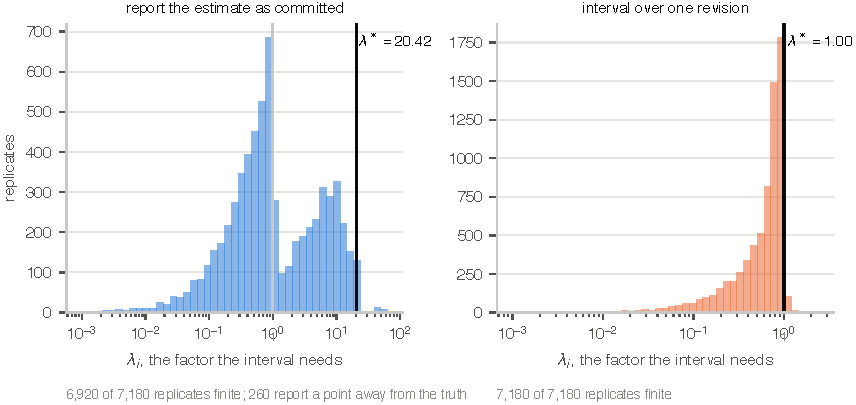
\includegraphics[width=\textwidth]{figs/f2_calibration.pdf}
\caption{The distribution of $\lambda_i$ over all 7{,}180 replicates of the one-wrong-claim cell,
for two procedures. Reporting the estimate as committed is bimodal: one group of problems is
roughly right, and a second group sits an order of magnitude away, which is what one false claim
does. Its 95th percentile is 20.4. The interval over one revision needs no stretching at all, so
its factor is 1.00.}
\end{figure}

The shape on the left is the finding behind the whole column. Committing to the analyst's graph does
not produce intervals that are a bit too narrow. It produces two populations: problems where the
false claim did not matter, and problems where the reported effect is simply somewhere else.

\subsection{Step 3. From the factor to a width, and then to a ratio}

Multiply each interval by $\lambda^{*}$ and average the resulting widths. That is the calibrated
width, in effect units. Then divide by the calibrated width of the procedure that discards the
knowledge entirely. The result is the number printed in the cell.

\begin{quoting}
At one wrong claim, $n = 1000$, semi-synthetic panel:

\smallskip
\begin{tabular}{@{}lrrr@{}}
\toprule
procedure & $\lambda^{*}$ & mean half-width & calibrated width \\
\midrule
report the estimate as committed & 20.416 & 0.3855 & 15.7397 \\
interval over one revision & 1.000 & 1.3064 & 2.6129 \\
discard the knowledge, whole class & 1.000 & 1.5361 & 3.0721 \\
\bottomrule
\end{tabular}

\smallskip
$15.7397 / 3.0721 = 5.123$. \qquad $2.6129 / 3.0721 = 0.851$.
\end{quoting}

Those are the two numbers in the middle column of the table. So the row that reports the estimate as
committed is a narrow interval, mean half-width 0.39 against 1.54 for the whole class, and it is the
most expensive of the three once you require it to be right.

\begin{figure}[h]
\centering
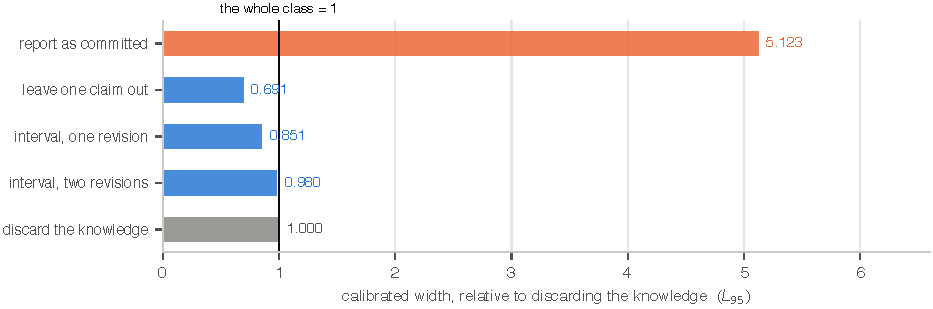
\includegraphics[width=\textwidth]{figs/f3_ratio.pdf}
\caption{The middle column of Panel B, as calibrated widths relative to discarding the knowledge.
Anything to the right of the line costs more than using no background knowledge at all.}
\end{figure}

\subsection{Why a number can exceed one, and what that means}

A procedure earns a number above one when its interval is narrow and centred in the wrong place.
Stretching happens about the interval's own midpoint, so a displaced midpoint has to be compensated
on both sides. Committing to a graph built on a false claim puts the midpoint at the effect that
graph implies, which is a different quantity from the one being estimated.

\begin{figure}[h]
\centering
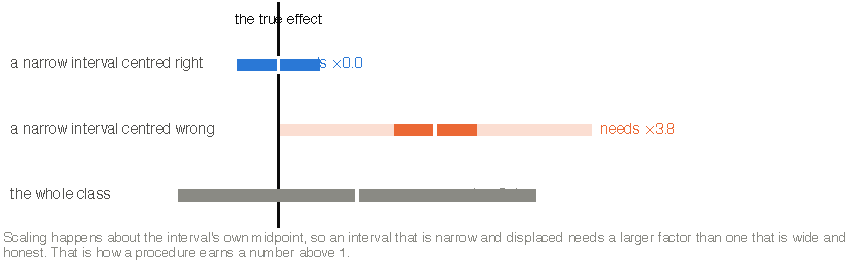
\includegraphics[width=\textwidth]{figs/f5_why_above_one.pdf}
\caption{Three intervals and the factor each needs. A narrow interval centred on the truth is cheap.
A narrow interval centred away from it is the most expensive object in the table. Schematic.}
\end{figure}

A value above one is therefore a strong statement, and it is the statement the table is making about
current practice: at one wrong claim, an analyst who reports the estimate their graph produced is
worse off than an analyst who never elicited any knowledge, by a factor of five.

\subsection{Reading the whole panel}

\begin{figure}[h]
\centering
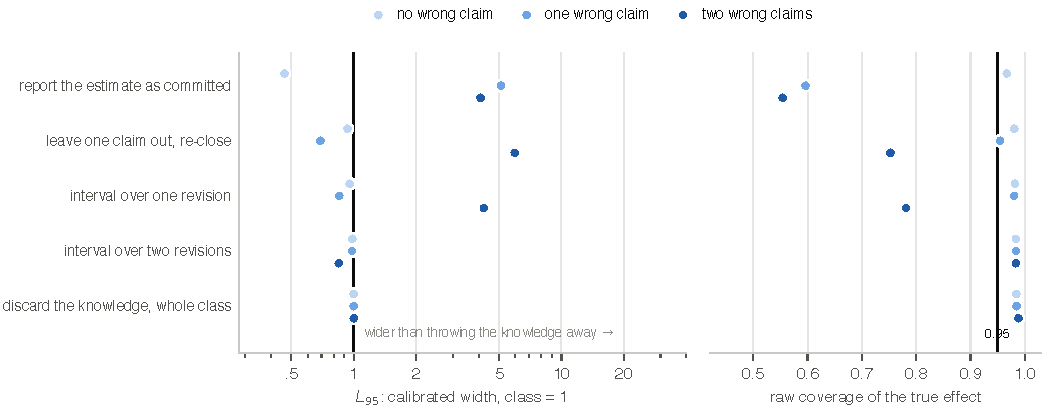
\includegraphics[width=\textwidth]{figs/f4_panelB.pdf}
\caption{Panel B as a chart. Left: the calibrated width of each procedure, with the whole class at
one. Right: the raw coverage each procedure achieved before any calibration. Semi-synthetic
parameters on published structures, $n = 1000$; 391, 359 and 131 problems over 23, 23 and 9
networks.}
\end{figure}

Five things are worth saying out loud from that picture.

The first column is a defeat and it has to be. When nothing is wrong, the committed report needs
0.464 and the interval over one revision needs 0.957, so the insurance costs about twice the width
when the knowledge is correct. A table in which the proposed method wins every column is a design
error, and a reviewer reads it as one.

One wrong claim is bought back cheaply. The committed report drops to 0.597 coverage, and the
interval over one revision covers 0.980 while needing 0.851 of the class width. It is also 15\,\% narrower than the procedure that uses no knowledge at all, which is the
reason the knowledge was worth eliciting in the first place.

Two wrong claims need two retractions. The interval over one revision fails at two wrong claims
(coverage 0.781, and a calibrated width of 4.234 that is worse than the class), and the interval
over two pays. The depth of the budget has to match the number of errors; there is no budget that is
free.

Retracting one claim far from the query is not the bargain it looks like. That row is the matched
negative control, and it costs more than doing nothing while buying four points of coverage. On the
semi-synthetic panel it is not inert, because a far retraction still propagates into the component
through the orientation rules. That prediction was recorded as partial rather than supported.

The free screen and the interval agree at this depth. The leave-one-out screen needs 0.691 at one
wrong claim against the interval's 0.851, and fails at two wrong claims exactly where the interval
over one revision fails. That is the tie the paper states as a property rather than hiding.

\subsection{Two cautions about the panel as printed}

\textbf{The three columns are three populations.} A problem enters the one-wrong-claim column only
if it has at least one local claim to falsify, and the two-wrong-claim column only if it has two and
they can be reversed consistently. That is why the counts fall from 391 to 359 to 131 and the
network count from 23 to 9. The populations are nested, and the counts are printed under the panel
for that reason. Comparing down a column is exact; comparing across a row is comparing three
different problem sets.

\textbf{The numbers depend on the sample size, and the table shows only one.} At $n = 20\,000$ the
committed report's number rises from 5.123 to 14.368, because more data makes a wrongly centred
interval narrower without moving it. The relative price of the interval improves from 0.851 to
0.758. The direction is the same and the magnitudes are not, so the sample size belongs in the
caption of any quotation.

\subsection{The definitions behind the row names}

\begin{center}\small
\begin{tabular}{@{}p{4.3cm}p{11.7cm}@{}}
\toprule
row & what the procedure does \\
\midrule
report the estimate as committed & Take the analyst's graph, read off the adjustment set the
generalised criterion gives, fit, report the ordinary 95\,\% interval. Where the graph commits to no
set, report the band over its own possible parent sets, which is the budget-zero interval. This is
the documented practice, and it is the default the table is arguing against \\
\addlinespace
leave one claim out, re-close, widen if it changes & For each claim in turn, drop it, close the graph
again under the orientation rules, recompute the committed set. If any of them changes the answer,
report the interval over one revision; otherwise report the committed estimate \\
\addlinespace
interval over one revision & The union of the estimates over every knowledge state within one
elementary revision of the analyst's claims, taken as an interval \\
\addlinespace
interval over two revisions & The same over two revisions \\
\addlinespace
discard the knowledge, whole class & The interval over every adjustment set the equivalence class
admits, using no background knowledge. It is the denominator of every cell, so it is 1.000 by
construction, and its raw coverage is printed to show that it is honest rather than merely wide \\
\bottomrule
\end{tabular}
\end{center}

Every row uses the same estimator and the same data. What differs between rows is only how many
revisions of the asserted knowledge the reported interval is willing to tolerate.
